\paragraph{Задание 3}
\subparagraph{Условие:}
Запустив Wireshark на захват, выполнить загрузку доступной в лабораторных условиях страницы (\url{www.bstu.by}, \url{www.iit.bstu.by} или др.). Остановить и сохранить захват. Для захваченных пакетов определить статистические данные:

\begin{itemize}
    \item процентное соотношение трафика разных протоколов в сети;
    \item среднюю скорость кадров/сек;
    \item среднюю скорость байт/сек;
    \item минимальный, максимальный и средний размеры пакета;
    \item степень использования полосы пропускания канала (загрузку сети).
\end{itemize}

\subparagraph{Решение:} \hspace{0pt}

Так как операционная система Debian 10, то скачиваю Wireshark через пакетный менеджер apt.

\begin{lstlisting}[language=Terminal,]
sudo apt update            # Обновление пакетов
sudo apt install wireshark # Установка Wireshark
\end{lstlisting}

Запускаем Wireshark от прав root.

\begin{lstlisting}[language=Terminal,]
sudo wireshark             # Запуск Wireshark от root прав
\end{lstlisting}

\subparagraph{1-ый подпункт}
Для показа процентноего соотношение трафика разных протоколов в сети
жму <<Statistics>>, затем <<Protocal Hierarchy>>.
Результат на рисунке \textbf{\ref{fig:3-1} (стр. \pageref{fig:3-1})}.

\subparagraph{2-ой и 3-ий подпункт}
Для показа средней скорости кадров/сек и средней скорости байт/сек
жму <<Statistics>>, затем <<Capture File Properties>>.
Результат на рисунке \textbf{\ref{fig:3-2} (стр. \pageref{fig:3-2})}.

\subparagraph{4-ый подпункт}
Для показа минимального, максимального и средного размеры пакета
жму <<Statistics>>, затем <<Packet Lengths>>.
Результат на рисунке \textbf{\ref{fig:3-4} (стр. \pageref{fig:3-4})}.

\subparagraph{5-ый подпункт}
Для показа степени использования полосы пропускания канала (загрузку сети)
жму <<Statistics>>, затем <<I/O Graph>>.
Результат на рисунке \textbf{\ref{fig:3-5} (стр. \pageref{fig:3-5})}.

\begin{figure}[!htp]
    \centering
    \begin{minipage}{.64\textwidth}
        \centering
        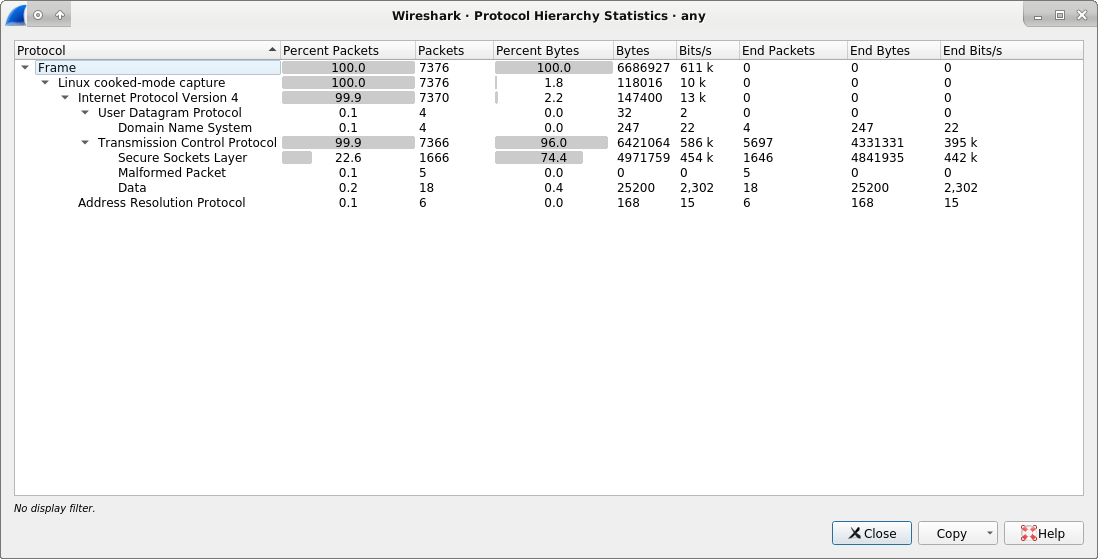
\includegraphics[width=.99\textwidth]
        {../_INCLUDES/main/task3/3-1.png}
        \caption{Statistics > Protocal Hierarchy}
        \label{fig:3-1}
    \end{minipage}
    \begin{minipage}{.34\textwidth}
        \centering
        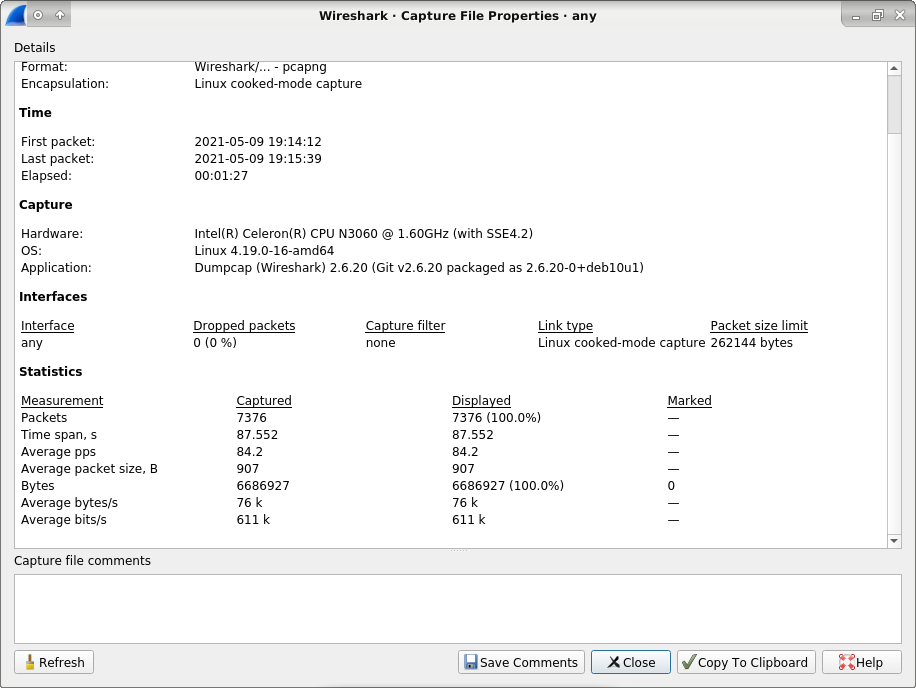
\includegraphics[width=.99\textwidth]
        {../_INCLUDES/main/task3/3-2.png}
        \caption{Statistics > Capture File Properties}
        \label{fig:3-2}
    \end{minipage}
\end{figure}

\begin{figure}[!htp]
    \centering
    \begin{minipage}{.64\textwidth}
        \centering
        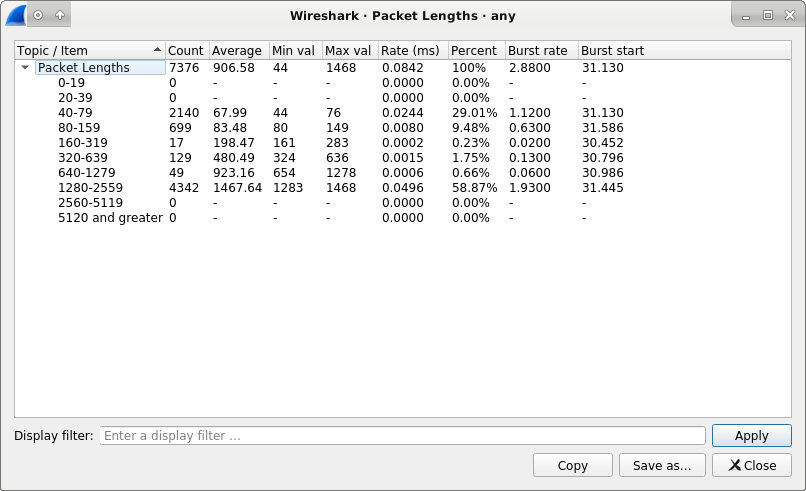
\includegraphics[width=.99\textwidth]
        {../_INCLUDES/main/task3/3-4.png}
        \caption{Statistics > Packet Lengths}
        \label{fig:3-4}
    \end{minipage}
    \begin{minipage}{.34\textwidth}
        \centering
        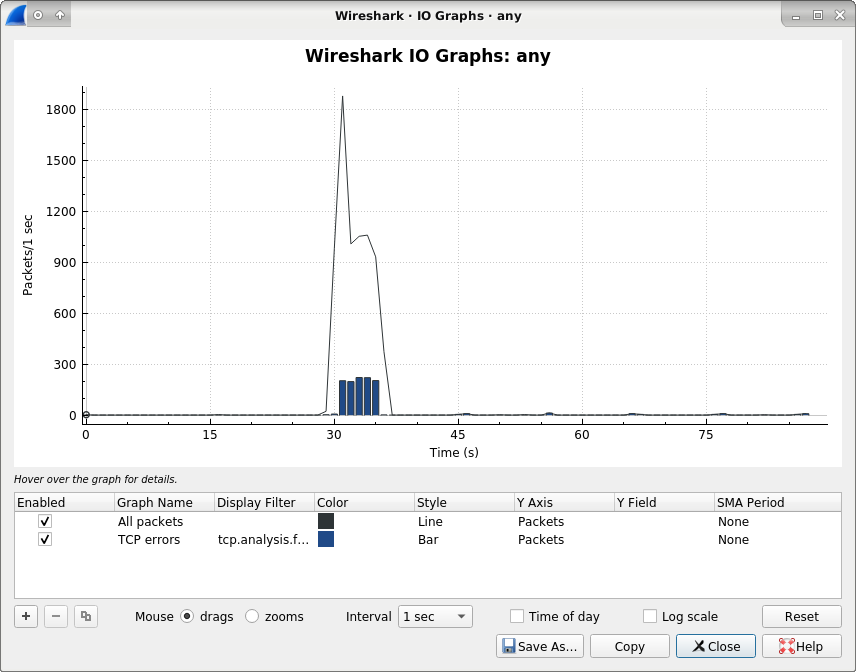
\includegraphics[width=.99\textwidth]
        {../_INCLUDES/main/task3/3-5.png}
        \caption{Statistics > I/O Graph}
        \label{fig:3-5}
    \end{minipage}
\end{figure}
